%*********************** INTRODUCTION **************
\chapter*{Introduction}Dans ce TP on va réaliser un asservissement de position ,on va utiliser pour cette manipulation la platine voir   la Figure 1.1.
\addcontentsline{toc}{chapter}{Introduction}

\begin{center}
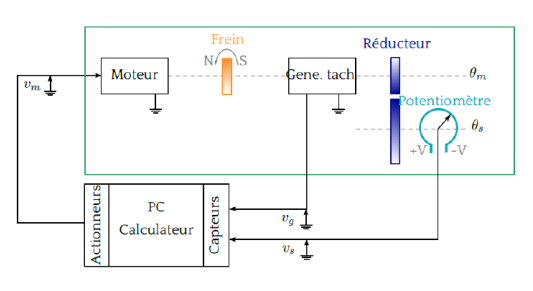
\includegraphics[scale=0.5]{fiiig1.png}
\captionof{figure}{\textit{Asservissement de position par calculateur}}
\label{fig1} 
\end{center}

Les valeurs numériques des coefficients connus sont:\\

 $K_e=10(V.tr^-1)$	 \hfill		$K_s=10(V.tr^-1)$	\hfill		$Kg=0.105(V.s.tr^-1)$ 